
\subsection{Efficiency studies from \decay{\Bd}{\jpsi\Kstarz}}
\label{sec:eff:cross}
It is expected that the selection in this analysis and the selection from the SM analysis in
Ref.~\cite{LHCb-CONF-2015-002} (detailed in LHCb-ANA-2013-97)
should yield a similar number of candidates for the decay \decay{\Bd}{\jpsi\Kstarz}.
Considering the high purity of the decay \decay{\Bd}{\jpsi\Kstarz} a fit is not necessary for a
first order approximation of relative efficiencies between the selection from
Ref.~\cite{LHCb-CONF-2015-002} and the one outlined in \Sect{sec:sel} are assessed by simply
counting the number of entries after the harshest cuts from both selections are applied to both
datasets offline.
Of course the BDTs and trigger lines are different.
Candidates are only counted if they are within $80\mev$ of the nominal \Bd mass, and if the dimuon
system has an invariant mass within $50\mev$ of the known \jpsi mass.
After all the cuts $\sim320000$ events remain in the SM dataset (which is what is observed after
the full fit in Ref.~\cite{LHCb-CONF-2015-002}), and $\sim290000$ candidates remain in the dataset
used in this analysis.
There are therefore only $\sim10\%$ fewer events in this selection, which is not surprising
considering this search is for a much rarer process than the SM \decay{\Bd}{\Kstarz\mumu}.

%Once again using the decay \decay{\Bd}{\jpsi\Kstarz}
Selected \decay{\Bd}{\jpsi\Kstarz} events are used to check that the selection was not biased in
terms of either year or magnet polarity.
No bias is observed in the number of events selected with respect to the luminosity delivered for
each 2011 MagUp, 2011 MagDown, 2012 MagUp, and 2012 MagDown.



\section{Blinded distributions}
\label{sec:results}

Figure~\ref{fig:res:mbvtau}, shows the \db candidate lifetime against \Bd
mass, it also shows the effect the uBDT cut has on the combinatorial background.
The lifetime of the \db candidate is also shown as a function of the \db mass, inside and outside
the \Bd signal region in Fig~\ref{fig:res:mxvtau}.

%\begin{figure}
  %\begin{center}
    %\subfloat[\label{fig:res:mbvtau:all}]{\includegraphics[width=0.48\textwidth]{mb_v_tau}}
    %\subfloat[\label{fig:res:mbvtau:bdt}]{\includegraphics[width=0.48\textwidth]{mb_v_tau_bdt}}
    %\caption{\small
      %Distributions of $\tau(\mumu)$ against $m(\Kstarz\mumu)$ for
      %candidates from data
      %\protect\subref{fig:res:mbvtau:all} with no cut, and
      %\protect\subref{fig:res:mbvtau:bdt} with a cut on the uBDT classifier.
      %The signal region has been blinded.
    %}
    %\label{fig:res:mbvtau}
  %\end{center}
%\end{figure}
%
%\begin{figure}
  %\begin{center}
    %\subfloat[\label{fig:res:mxvtau:all}]{\includegraphics[width=0.48\textwidth]{mx_v_tau}}
    %\subfloat[\label{fig:res:mxvtau:sig}]{\includegraphics[width=0.48\textwidth]{mx_v_tau_sig}}\\
    %\subfloat[\label{fig:res:mxvtau:bdtall}]{\includegraphics[width=0.48\textwidth]{mx_v_tau_bdt}}
    %\subfloat[\label{fig:res:mxvtau:bdtsig}]{\includegraphics[width=0.48\textwidth]{mx_v_tau_sig}}
    %\caption{\small
      %Distributions of $\tau(\mumu)$ against $m(\mumu)$ for \db candidates from data in the
      %\protect\subref{fig:res:mxvtau:all} upper mass sideband, and
      %\protect\subref{fig:res:mxvtau:sig} signal region (without the uBDT applied).
      %The Figs.~\protect\subref{fig:res:mxvtau:bdtall} and \protect\subref{fig:res:mxvtau:bdtsig} show the
      %same, but with uBDT cut applied (blank plots emphasize the analysis is blind).
      %%\emph{Blank plots will be filled in after unblinding.}
    %}
    %\label{fig:res:mxvtau}
  %\end{center}
%\end{figure}




Combinatorial background
is estimated with the following procedure for each of the lifetime regions:
\begin{itemize}
  \item Perform fit using an exponential function to the upper and lower mass sidebands of the \Bd
    candidate mass spectrum.  Sideband regions are defined by the areas outside of $60\mev$ from
    the known \Bd mass (approximately $3\,\sigma$).
    The fits are shown in \Fig{fig:res:comb}.
  \item Calculate the integral of the background function (exponential) in the signal region
    (within $60\mev$ of the known \Bd mass).
    Let the value of the integral be $m$.
  \item Take $m$ events from the upper sideband, and plot the mass of each dimuon candidate that
    forms the \Bd candidates.
\end{itemize}
The resulting invariant dimuon mass spectrum is shown in \Fig{fig:res:comb}; in the prompt case
there is an average of 1.8 events in each bin, in the displaced region the number is nearer 0.2.
Using bin widths comparable to the signal window size ($20\mev$) it is seen that the estimated
number of events per bin is always five or less, with an average of less than one event per bin.
A more detailed study will be performed below in wide bins as part of the unblinding strategy.


%\begin{figure}
  %\begin{center}
    %\subfloat[\label{fig:comb:fit0}]{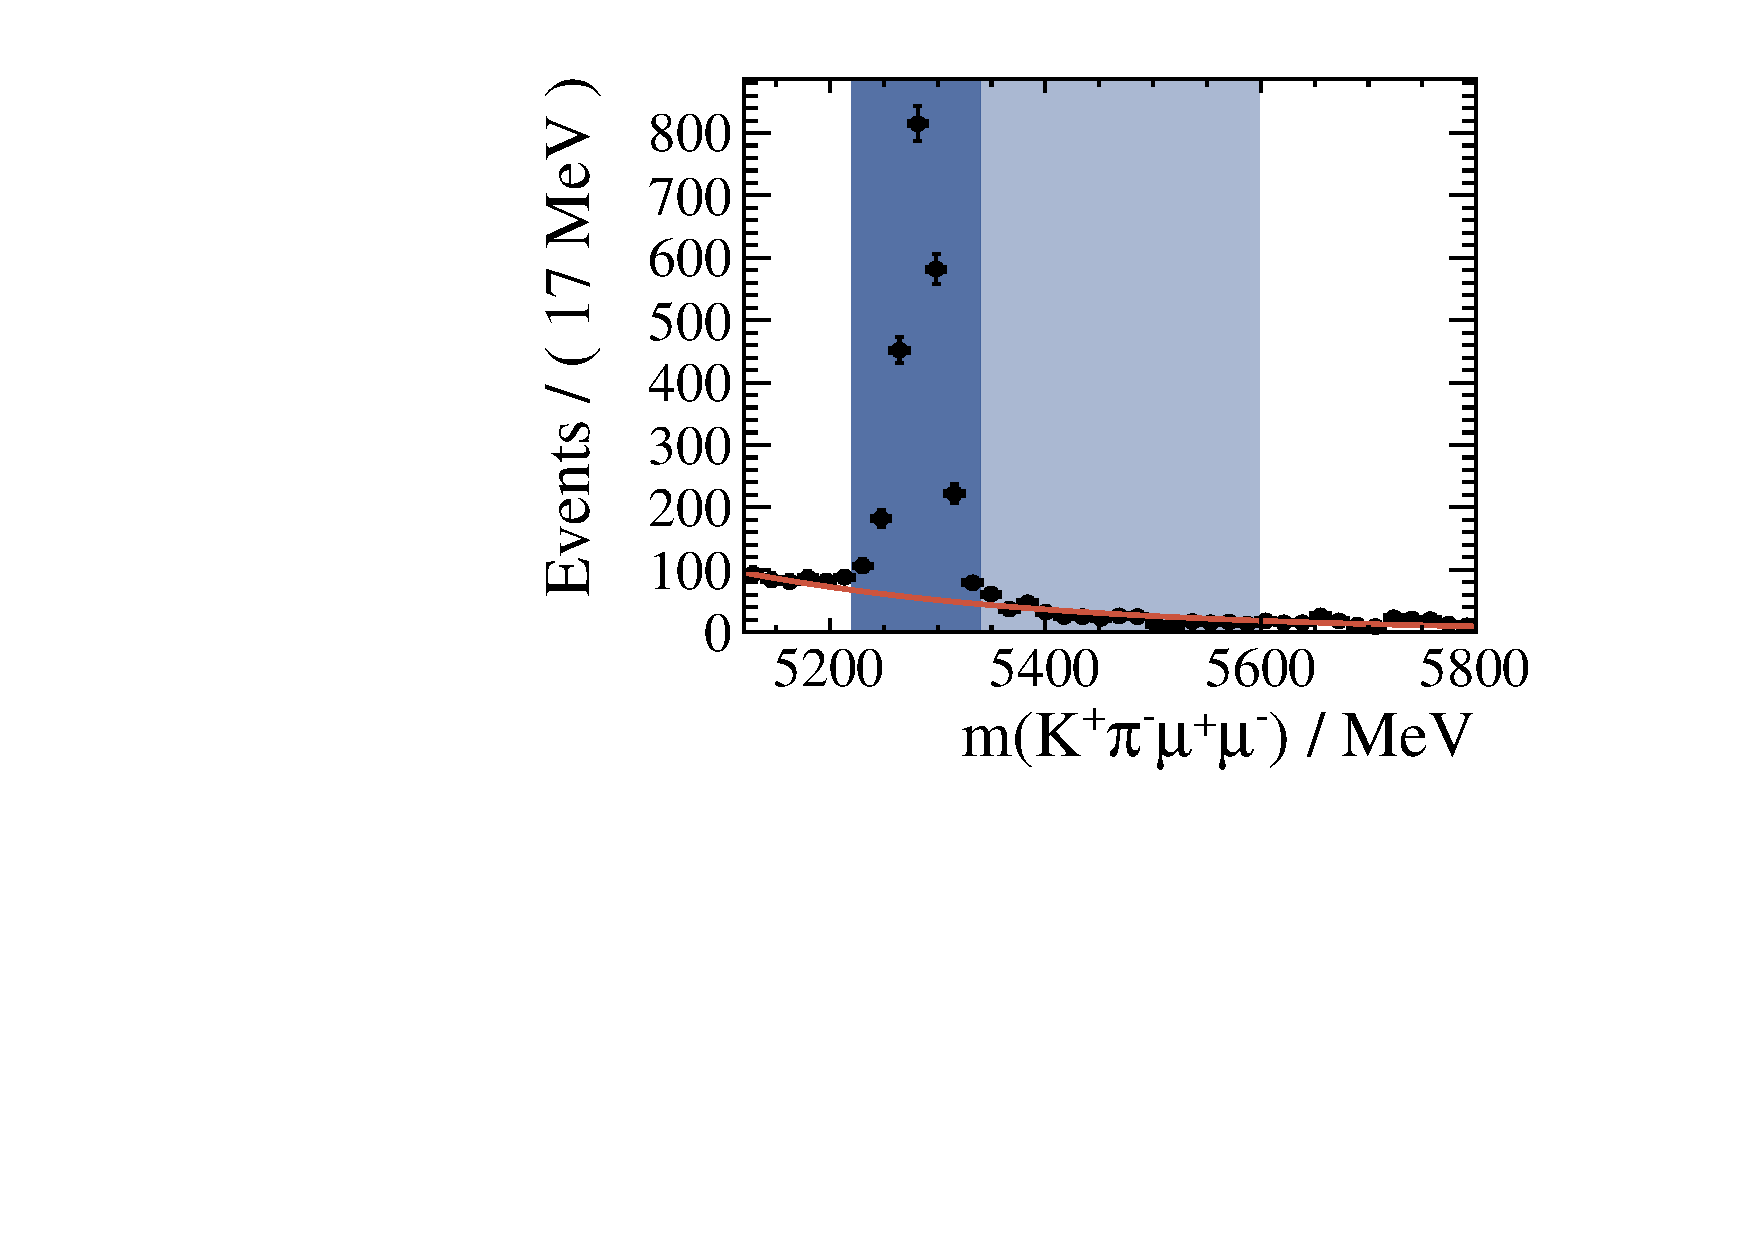
\includegraphics[width=0.48\textwidth]{combinatorial_prompt_fit}}
    %\subfloat[\label{fig:comb:fit1}]{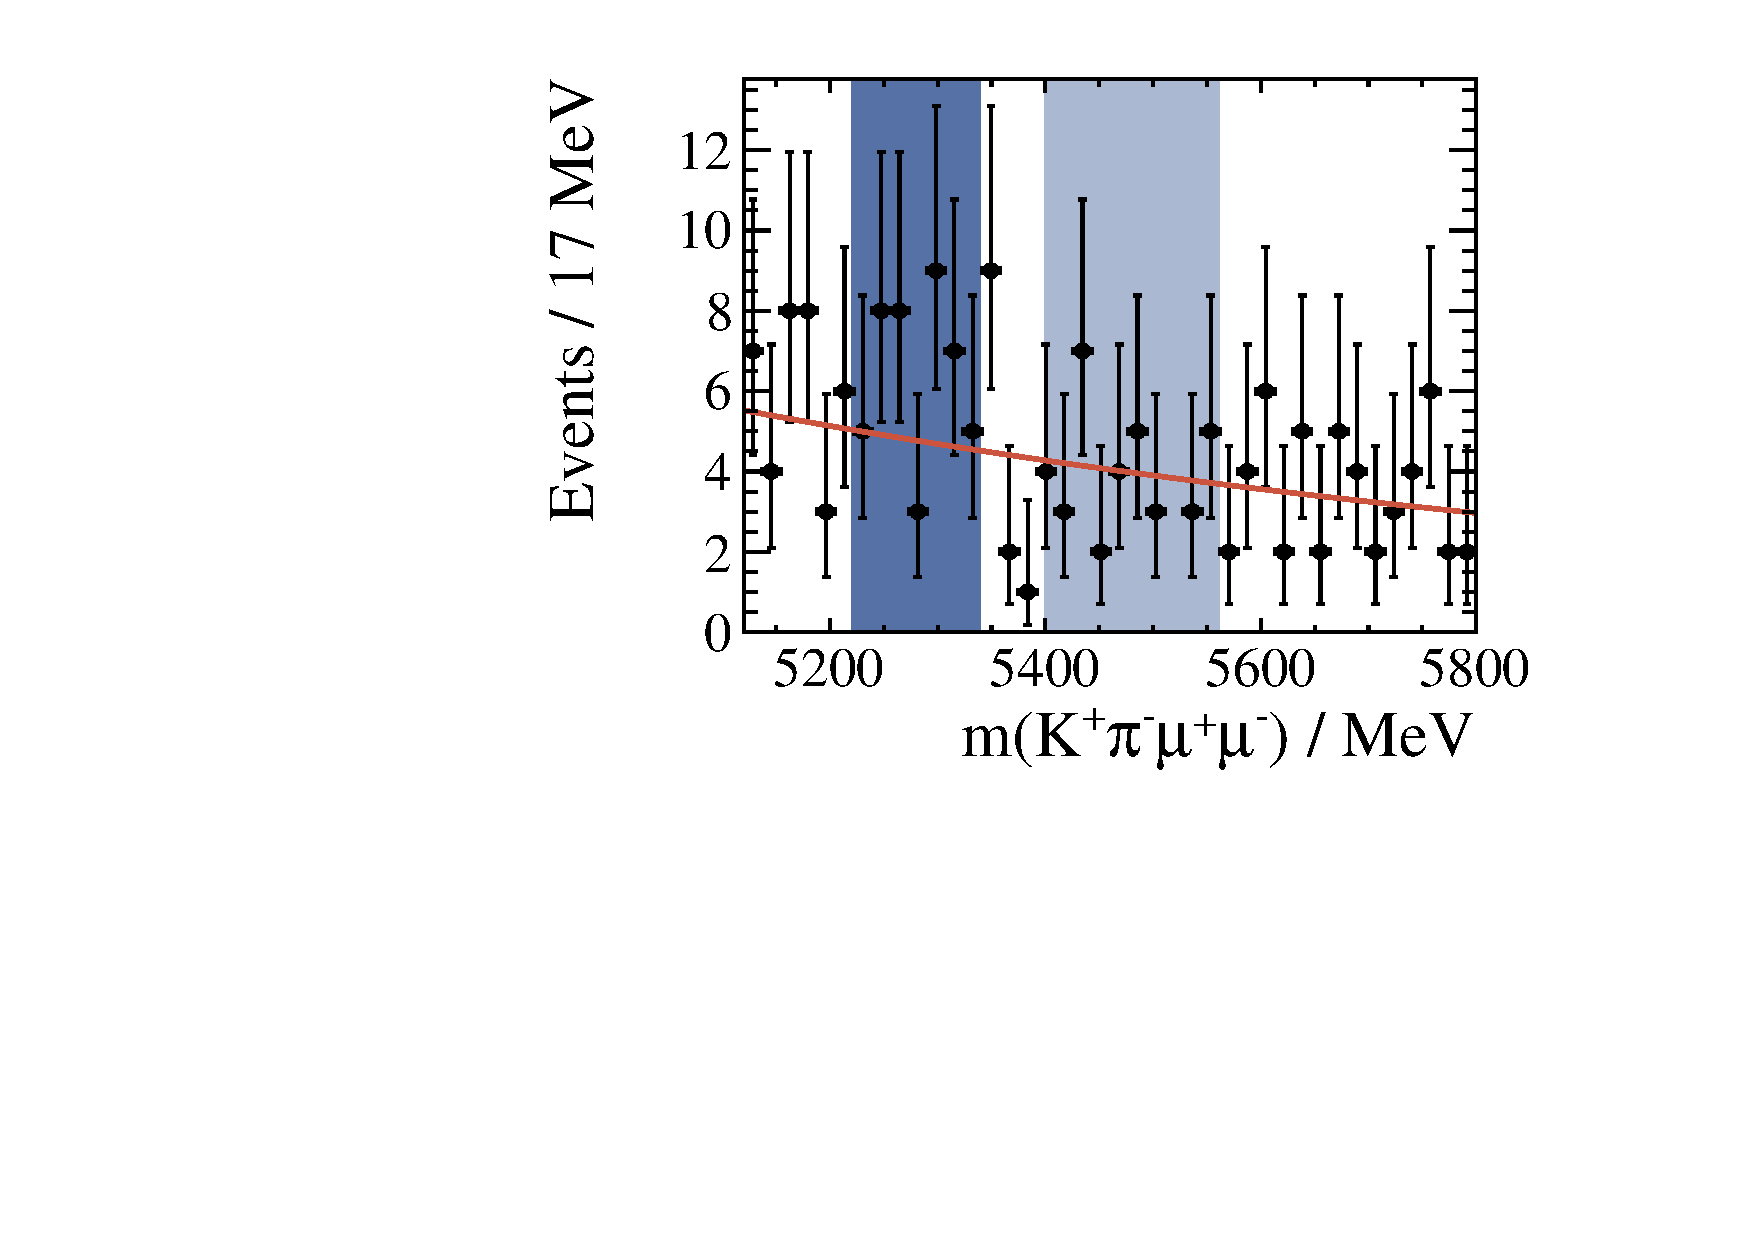
\includegraphics[width=0.48\textwidth]{combinatorial_displaced_fit}}\\
    %\subfloat[\label{fig:res:comb:pr}]{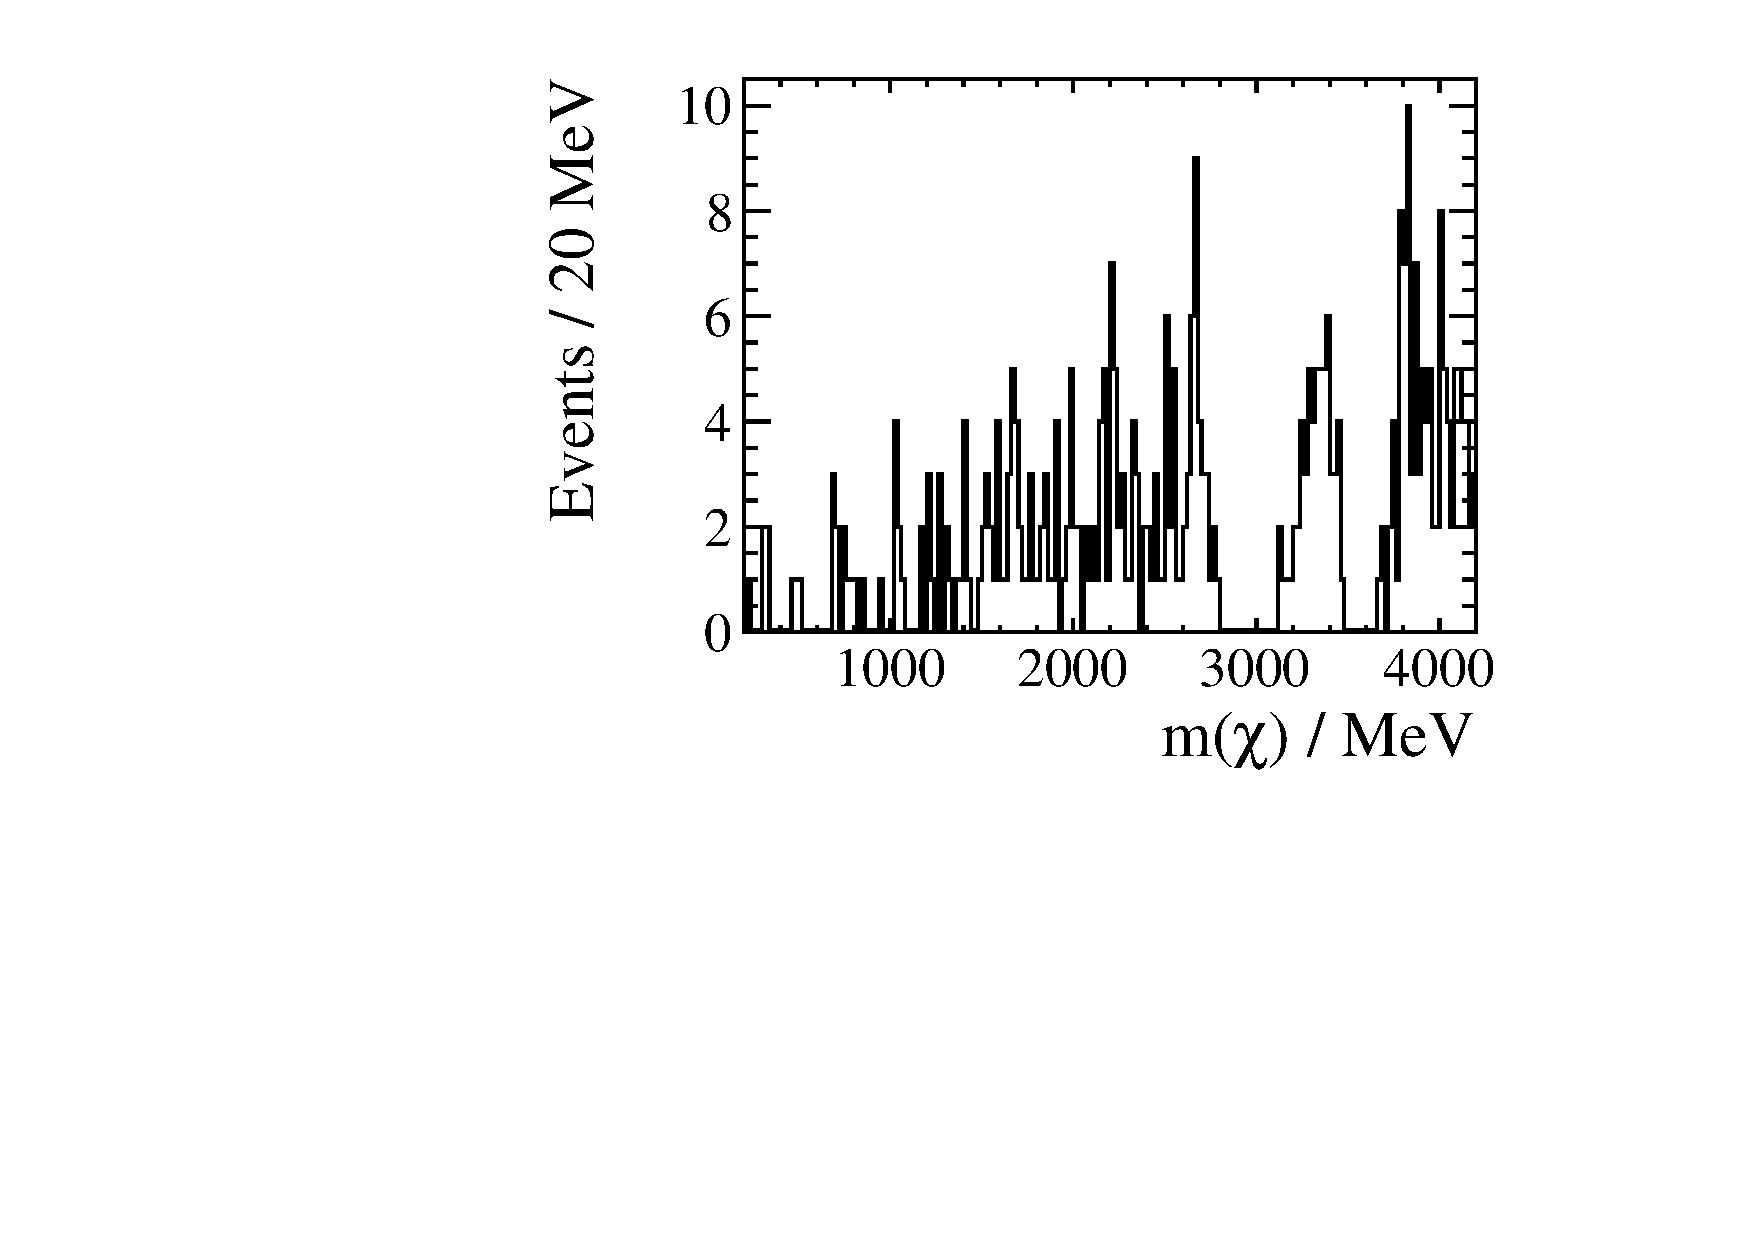
\includegraphics[width=0.48\textwidth]{combinatorial_prompt}}
    %\subfloat[\label{fig:res:comb:di}]{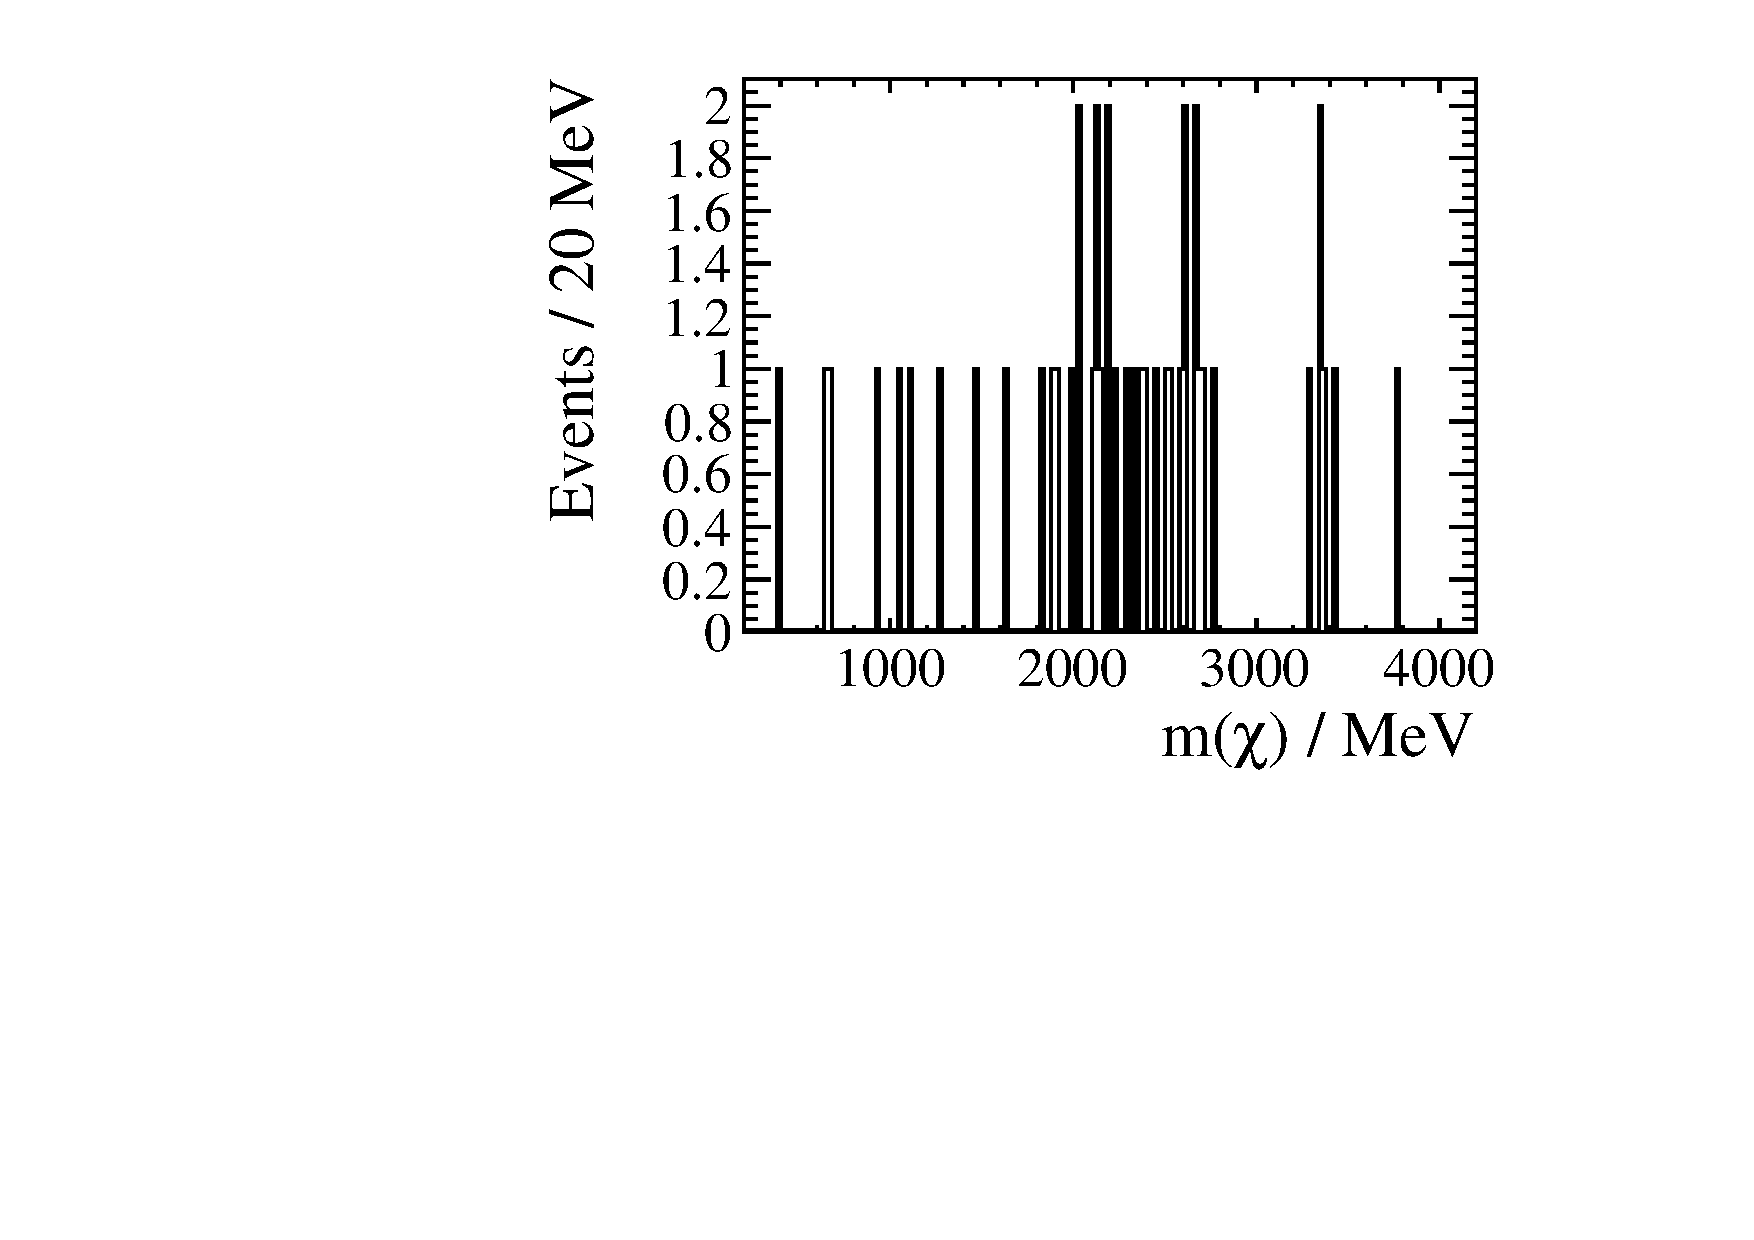
\includegraphics[width=0.48\textwidth]{combinatorial_displaced}}
    %\caption{\small
      %Fits to the prompt and displaced regions are shown in
      %\protect\subref{fig:comb:fit0} and
      %\protect\subref{fig:comb:fit1} respectively; where the dark blue box indicates the signal
      %region, and the lighter blue indicates the upper sideband which has the same area as the
      %background contribution to the signal region.
      %Combinatorial background estimations from data, as described in text are shown in
      %\protect\subref{fig:res:comb:pr} the prompt region, and
      %\protect\subref{fig:res:comb:di} the displaced region.
      %Each bin is $20\mev$ wide, which is comparable to the width of the signal region.
    %}
    %\label{fig:res:comb}
  %\end{center}
%\end{figure}








\section{Unblinding the data}

This analysis is performed blindly, and as such a strategy for the unblinding procedure mus be
laid out.
Firstly the \Bd mass peak will be unblinded in the prompt region for various ranges in \qsq, which
can be compared with the \sm yields.

\subsection{Step 1: normalization mode}
The first step in the unblinding procedure is to check the  yield of the normalization channel
\btokstrmumu in the range $1.1<\qsq<6.0\gevgev$ and compare with the yield from the SM analysis,
which is outlined in LHCb-ANA-2013-093.
The yield of the normalization channel in this analysis was calculated using the selection outlined
in \Sect{sec:sel} and only in the prompt region (as defined by the resolutions in \Fig{fig:eff:res}),
and multiple candidates were removed at random.
The final fit to the \btokstrmumu candidates was made using the same mass model, and fit results as
in LHCb-ANA-2013-097.
The signal model is constructed from the sum of two Gaussian functions with power-law tail on the
low-mass side.
The background is a simple exponential where the exponent is allowed to float freely.
The resulting dataset and fit is shown in \Fig{fig:fit126}.

%\begin{figure}
  %\begin{center}
    %\includegraphics[width=0.48\textwidth]{normChannel_126}
    %\caption{
      %Fit to the invariant mass spectrum of the \Bd candidates in selected data in the range
      %$1.1<\qsq<6.0\gevgev$.
      %The signal model is the sum of two Gaussian functions with power-law tails on the low-mass
      %side with parameters taken from LHCb-ANA-2013-097, the background model is a decaying
      %exponential.
      %This fit results in a signal yield of $(653\pm29)$ compared to approximately 625 in the SM
      %analysis; for more in depth numbers, please refer to Table~\protect\ref{tab:db:nums126}.
    %}
    %\label{fig:fit126}
  %\end{center}
%\end{figure}


After unblinding the region $1.1<\qsq<6.0\gevgev$, other prompt \qsq regions were also looked at to
determine the ratio of BDT selection efficiencies
$\varepsilon_\mathrm{BDT}^\mathrm{\qsq bin} / \varepsilon_\mathrm{BDT}^{\decay{\Bd}{\jpsi\Kstarz}}$
in different \qsq bins (those used in the SM analysis), for data and simulation.
To determine these efficiencies, we apply the pre-BDT selection and perform a fit to determine the $B$ yield.  Next, we apply the BDT cut and perform a second fit, then take the ratio of the $B$ yields.
This comparison is shown in \Fig{fig:bdtEffRatio}.
Data and simulation are shown to be in good agreement, centred around unity with about 5--10\% precision.
This approach ignores the fact that there may be some small peaking background component that gets counted as signal pre-BDT cut, but is removed by the BDT.  Note, however, that in the $\varepsilon_\mathrm{BDT}^\mathrm{\qsq bin} / \varepsilon_\mathrm{BDT}^{\decay{\Bd}{\jpsi\Kstarz}}$ ratio, only the difference in peaking background contributions matters.  Given that we explicitly veto all peaking backgrounds that are visible in the various 2-body mass combinations, we do not expect any peaking background contributions at the level of the statistical precision of this test.

%\begin{figure}
  %\begin{center}
    %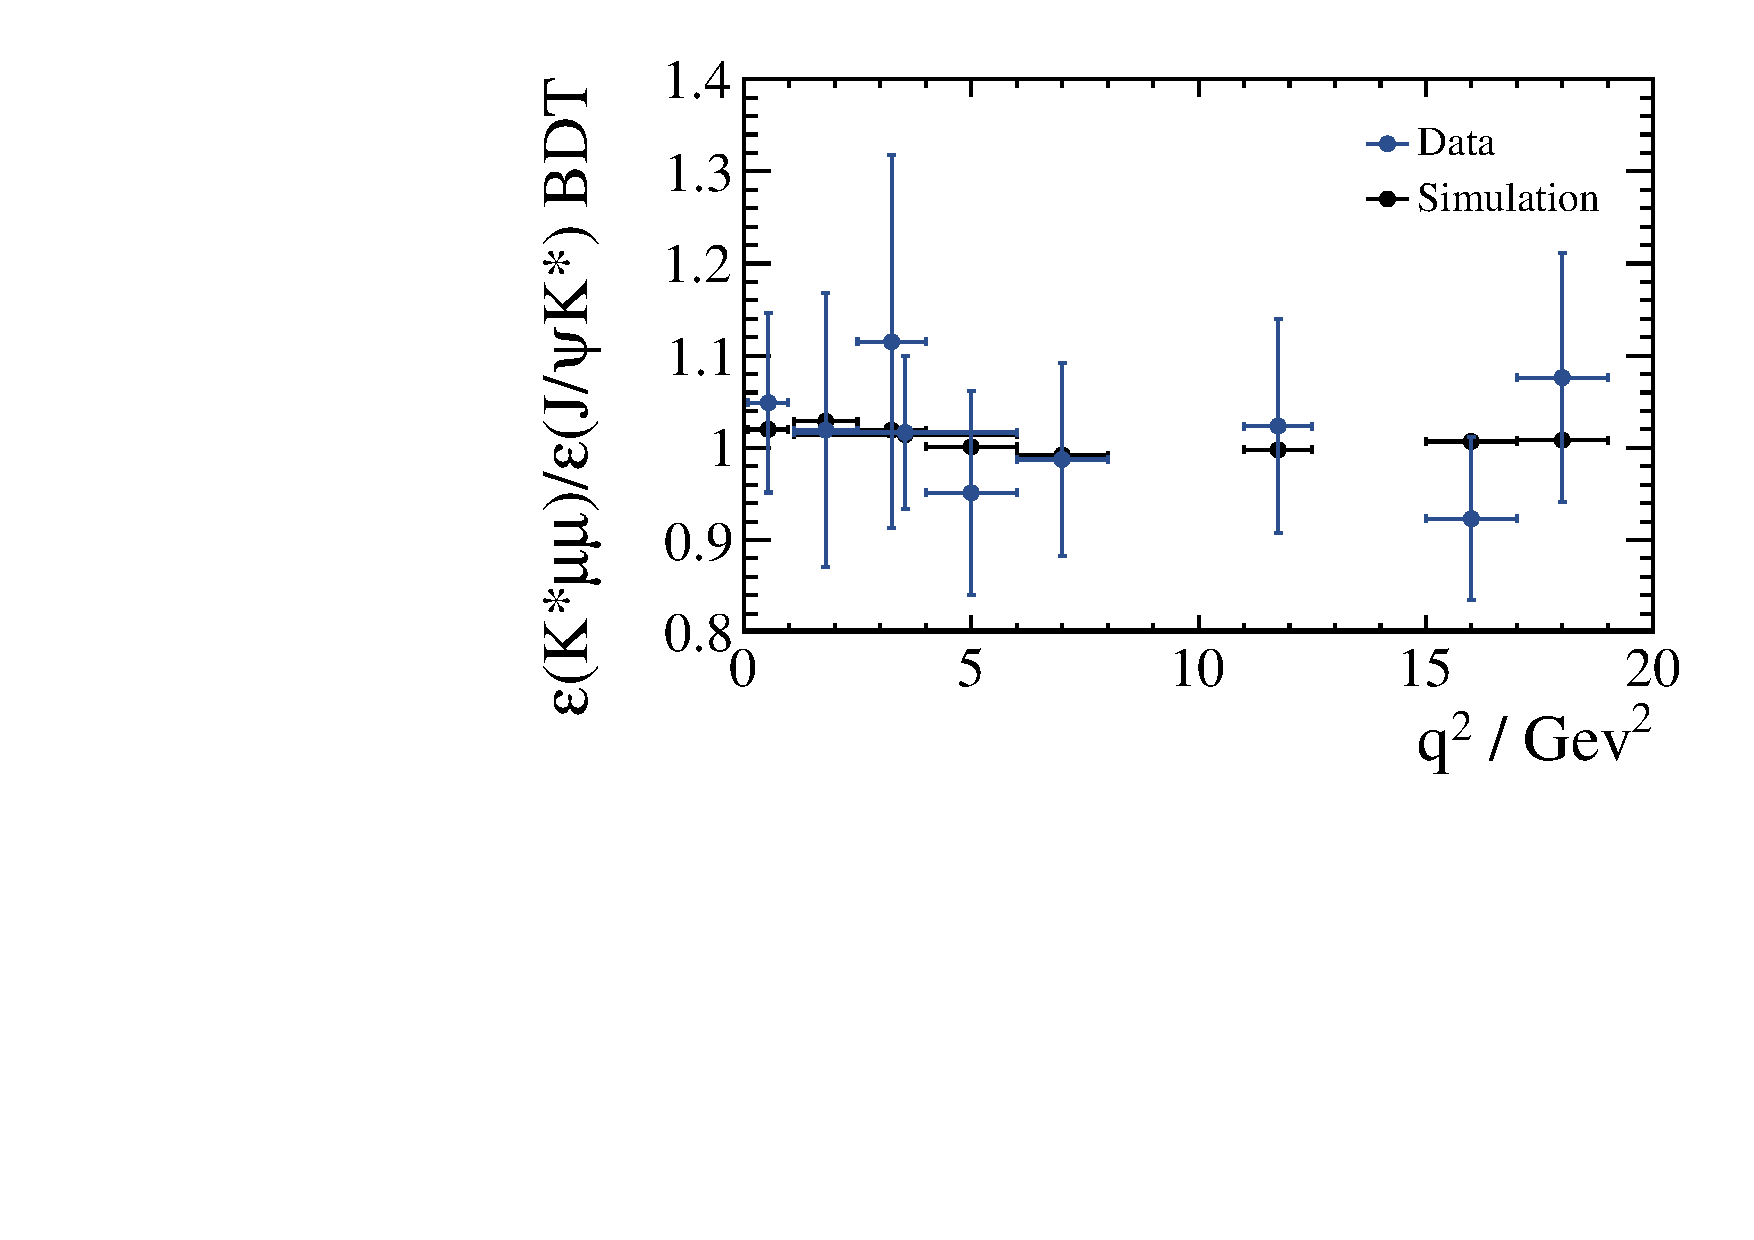
\includegraphics[width=0.48\textwidth]{bdtEffRatio}
    %\caption{
      %Ratio of the efficiencies of the BDT selection for a range of \qsq bins, as used in the SM
      %\btokstrmumu analysis, with respect to the efficiency for \decay{\Bd}{\jpsi\Kstarz}.
      %Data and simulation are shown to be in good agreement.
    %}
    %\label{fig:bdtEffRatio}
  %\end{center}
%\end{figure}
